\chapter{Thực Nghiệm Và Đánh Giá}

\section{Mục tiêu và nguyên tắc đánh giá}

Thực nghiệm nhằm kiểm tra ba lớp khác nhau: (1) tính đúng của thuật toán và luật
chuyển trạng thái; (2) khả năng chạy trên graph đóng gói thật; (3) hành vi tương
đối của các heuristic truy tìm. Một ca test đạt không tự động chứng minh hiệu quả
trên người dùng thật; một benchmark bot cũng không chứng minh chính sách tối ưu.
Các kết luận dưới đây được giới hạn theo đúng bằng chứng của từng phép đo.

Các kết quả trong chương được chạy lại ngày 24/10/2026 trên máy phát triển dùng
Python 3.11. Thời gian là thời gian thực đo của một lần chạy, chịu ảnh hưởng tải
CPU, bộ nhớ và cache; vì vậy chỉ dùng để mô tả cấu hình hiện tại.

\section{Chiến lược kiểm thử}

\subsection{Phân bố 112 ca kiểm thử}

\begin{table}[H]
\centering
\caption{Số ca kiểm thử theo mô-đun}
\begin{tabularx}{\linewidth}{Y r Y}
\toprule
\textbf{Tệp} & \textbf{Số test} & \textbf{Trọng tâm} \\
\midrule
\texttt{test\_chase.py} & 38 & Luật, tập niềm tin, ba chiến thuật, terminal priority \\
\texttt{test\_services.py} & 17 & Nạp graph, bbox, lỗi mạng/dữ liệu, cache \\
\texttt{test\_chase\_maps.py} & 11 & Sân, chia cạnh, seed, GraphML gián đoạn \\
\texttt{test\_tsp.py} & 11 & Held--Karp, ba kiểu kết thúc, ma trận bất đối xứng \\
\texttt{test\_chase\_app.py} & 9 & AppTest cho điều khiển và trạng thái ván \\
\texttt{test\_app.py} & 7 & Luồng giao diện định tuyến \\
\texttt{test\_app\_modes.py} & 7 & Chuyển chế độ và bảo toàn session state \\
\texttt{test\_shortest\_path.py} & 7 & Dijkstra, đa cạnh, vô hướng tới đích, oracle ngẫu nhiên \\
\texttt{test\_heuristics.py} & 3 & Nearest-neighbor và 2-opt \\
\texttt{test\_preload.py}, \texttt{test\_pbf\_preload.py} & 2 & An toàn khi chuẩn bị dữ liệu \\
\midrule
\textbf{Tổng} & \textbf{112} & \textbf{Tất cả đạt} \\
\bottomrule
\end{tabularx}
\end{table}

Lệnh \texttt{python -m unittest discover -s tests -q} chạy 112 test trong
18,431 giây và trả về \texttt{OK}. Một số test cố ý đưa metadata hoặc Pickle sai
để kiểm tra đường lỗi; traceback log trong các trường hợp này là dữ liệu test,
không phải test thất bại.

\subsection{Các nhóm trường hợp biên}

Đối với Dijkstra, test bao phủ nguồn bằng đích, đích không tới được, cạnh song
song, graph có hướng, trọng số sai và so sánh với NetworkX trên graph ngẫu nhiên.
Đối với Held--Karp, test bao phủ $n=1$, tuyến mở, điểm cuối cố định, chu trình,
ma trận bất đối xứng, chi phí vô hạn và đối chiếu vét cạn ở kích thước nhỏ.

Đối với trò chơi, các ca quan trọng gồm: bắt và thoát cùng nút thì bắt ưu tiên;
thoát ở lượt cuối vẫn thắng trước timeout; máy bắt sau khi di chuyển; không cho đi
sau terminal; loại nút đội máy khỏi niềm tin khi người trốn sống; policy nhận cùng
quan sát phải cho cùng quyết định dù trạng thái ẩn khác; và mọi bước đi không vượt
ngân sách. Các test này gắn trực tiếp với bất biến, không chỉ với dòng hiển thị.

\section{Smoke test định tuyến trên graph thật}

Kịch bản offline dùng năm địa điểm: Đại học Phenikaa, Sân vận động Mỹ Đình, Công
viên Cầu Giấy, đường Thanh Niên bên Hồ Tây và Đinh Tiên Hoàng bên Hồ Hoàn Kiếm.
Khoảng cách snap lớn nhất từ tọa độ mẫu tới graph là 217,85 m. Cùng một tập điểm
được tối ưu theo hai trọng số.

\begin{table}[H]
\centering
\caption{Kết quả smoke test năm địa điểm ngày 24/10/2026}
\begin{tabularx}{\linewidth}{p{3.0cm}Y r r r r}
\toprule
\textbf{Mục tiêu} & \textbf{Thứ tự chỉ số} & \textbf{Quãng đường} &
\textbf{Thời gian} & \textbf{Dijkstra} & \textbf{Held--Karp} \\
\midrule
Chiều dài & 0--1--2--4--3 & 26,276 km & 32,59 phút & 1,028 s & 0,174 ms \\
Thời gian & 0--1--2--4--3 & 27,049 km & 29,93 phút & 0,921 s & 0,136 ms \\
\bottomrule
\end{tabularx}
\end{table}

Graph nạp trong 9,845 giây ở lần chạy này. Cả hai mục tiêu cho cùng thứ tự ghé,
nhưng đường chi tiết khác: tối ưu thời gian dài hơn 0,773 km và nhanh hơn 2,66
phút theo trọng số ước tính. Điều này cho thấy tiêu chí tác động tới việc chọn
đoạn đường ngay cả khi thứ tự điểm không đổi.

Thời gian Held--Karp dưới 0,2 ms nhỏ hơn nhiều so với Dijkstra gần một giây. Kết
quả phù hợp với kiến trúc: chỉ có năm điểm trong bài toán quy hoạch động, trong
khi Dijkstra làm việc trên graph hàng trăm nghìn nút. Không nên suy rộng thời
gian này cho 10 điểm hay cho phần cứng khác mà không đo lại.

\section{So sánh thuật toán chính xác và heuristic trên tầng thứ tự ghé}
\label{sec:benchmark-tsp}

\subsection{Thiết kế phép đo}

Smoke test ở mục trước chỉ dùng năm địa điểm và một lần chạy, nên chưa đủ để nói
về hai điều mà Chương~2 đã tuyên bố: Held--Karp tăng theo $2^n$, còn hai heuristic
không có bảo đảm tối ưu. Vì vậy nhóm bổ sung một benchmark riêng cho tầng thứ tự
ghé, chạy bằng \texttt{scripts/benchmark\_tsp.py}.

Thiết kế như sau. Mười một địa điểm đầu trong \texttt{POPULAR\_LOCATIONS} được
snap vào graph Hà Nội đóng gói, khoảng cách snap lớn nhất là 263,22 m. Ma trận chi
phí có hướng đầy đủ $11\times 11$ được tính một lần; với mỗi $n$ từ 4 đến 11, phép
đo dùng ma trận con $n\times n$ của chính ma trận đó. Nhờ vậy ba thuật toán nhận
đúng cùng một dữ liệu đầu vào và phần Dijkstra không lẫn vào thời gian của tầng tổ
hợp. Mỗi cấu hình được chạy lặp năm lần; bảng báo thời gian trung bình.

Với mỗi $n$, cả ba kiểu kết thúc đều được đo. Ở kiểu điểm cuối cố định, điểm cuối
luôn là điểm cuối cùng của tập con. Khoảng cách chất lượng của một heuristic được
định nghĩa là
\[
  \mathrm{gap} = \left(\frac{C_{\text{heuristic}}}{C_{\text{Held--Karp}}}-1\right)\times 100\%,
\]
hợp lệ vì Held--Karp là tối ưu chính xác trên cùng ma trận, nên mẫu số chính là
chi phí nhỏ nhất.

\subsection{Chất lượng nghiệm}

\small
\setlength{\tabcolsep}{4pt}
\begin{longtable}{r l r r r r r}
\caption{Chi phí nghiệm theo mục tiêu quãng đường; gap so với Held--Karp}
\label{tab:tsp-quality}\\
\toprule
\textbf{Điểm} & \textbf{Kiểu kết thúc} & \textbf{Held--Karp} & \textbf{NN} &
\textbf{Gap NN} & \textbf{NN + 2-opt} & \textbf{Gap 2-opt} \\
 & & (km) & (km) & (\%) & (km) & (\%) \\
\midrule
\endfirsthead
\toprule
\textbf{Điểm} & \textbf{Kiểu kết thúc} & \textbf{Held--Karp} & \textbf{NN} &
\textbf{Gap NN} & \textbf{NN + 2-opt} & \textbf{Gap 2-opt} \\
 & & (km) & (km) & (\%) & (km) & (\%) \\
\midrule
\endhead
4 & Tuyến mở & 22,394 & 22,394 & 0,00 & 22,394 & 0,00 \\
4 & Điểm cuối cố định & 22,394 & 22,394 & 0,00 & 22,394 & 0,00 \\
4 & Chu trình & 37,068 & 37,081 & 0,03 & 37,068 & 0,00 \\
5 & Tuyến mở & 26,276 & 26,509 & 0,89 & 26,276 & 0,00 \\
5 & Điểm cuối cố định & 26,509 & 26,509 & 0,00 & 26,509 & 0,00 \\
5 & Chu trình & 40,343 & 41,417 & 2,66 & 40,343 & 0,00 \\
6 & Tuyến mở & 33,757 & 33,757 & 0,00 & 33,757 & 0,00 \\
6 & Điểm cuối cố định & 33,757 & 33,757 & 0,00 & 33,757 & 0,00 \\
6 & Chu trình & 52,566 & 54,806 & 4,26 & 52,566 & 0,00 \\
7 & Tuyến mở & 35,384 & 35,384 & 0,00 & 35,384 & 0,00 \\
7 & Điểm cuối cố định & 40,927 & 42,206 & 3,13 & 40,927 & 0,00 \\
7 & Chu trình & 53,545 & 56,433 & 5,39 & 54,369 & 1,54 \\
8 & Tuyến mở & 35,384 & 35,384 & 0,00 & 35,384 & 0,00 \\
8 & Điểm cuối cố định & 41,171 & 43,992 & 6,85 & 41,171 & 0,00 \\
8 & Chu trình & 53,981 & 56,433 & 4,54 & 54,369 & 0,72 \\
9 & Tuyến mở & 40,905 & 40,905 & 0,00 & 40,905 & 0,00 \\
9 & Điểm cuối cố định & 43,612 & 43,612 & 0,00 & 43,612 & 0,00 \\
9 & Chu trình & 56,087 & 61,954 & 10,46 & 56,087 & 0,00 \\
10 & Tuyến mở & 45,946 & 45,946 & 0,00 & 45,946 & 0,00 \\
10 & Điểm cuối cố định & 49,580 & 53,370 & 7,64 & 49,580 & 0,00 \\
10 & Chu trình & 58,153 & 66,995 & 15,20 & 60,359 & 3,79 \\
11 & Tuyến mở & 47,056 & 47,056 & 0,00 & 47,056 & 0,00 \\
11 & Điểm cuối cố định & 55,512 & 66,351 & 19,53 & 57,718 & 3,97 \\
11 & Chu trình & 59,368 & 68,105 & 14,72 & 61,573 & 3,71 \\
\midrule
\multicolumn{4}{l}{\textbf{Trung bình 24 cấu hình}} & \textbf{3,97} & &
\textbf{0,57} \\
\multicolumn{4}{l}{\textbf{Lớn nhất}} & \textbf{19,53} & & \textbf{3,97} \\
\bottomrule
\end{longtable}
\normalsize
\setlength{\tabcolsep}{6pt}

Kết quả cho ba nhận định. Thứ nhất, heuristic \textbf{không} sai một cách hiển
nhiên: ở tuyến mở, nearest-neighbor trùng nghiệm tối ưu trong cả tám kích thước.
Nguyên nhân là tuyến mở không bị ràng buộc điểm cuối, nên lựa chọn tham lam
``đi tiếp tới điểm gần nhất'' phù hợp với cấu trúc địa lý trải dài của tập điểm
mẫu.

Thứ hai, khoảng cách xuất hiện ngay khi có thêm ràng buộc. Với chu trình và điểm
cuối cố định, nearest-neighbor lệch tới 15,20\% và 19,53\%. Đây đúng là điểm yếu
đã nêu trong lý thuyết: quyết định tham lam ban đầu không tính tới chi phí quay
về hoặc chi phí phải kết thúc tại một điểm định sẵn \cite{rosenkrantz1977}.

Thứ ba, 2-opt thu hẹp phần lớn khoảng cách nhưng không xóa được: gap trung bình
giảm từ 3,97\% xuống 0,57\%, còn gap lớn nhất giảm từ 19,53\% xuống 3,97\%. Trong
17/24 cấu hình, 2-opt chạm đúng nghiệm tối ưu, nhưng 7 cấu hình còn lại vẫn kẹt ở
cực tiểu cục bộ. Quan sát này là bằng chứng trực tiếp cho phát biểu ``heuristic
không có bảo đảm tối ưu toàn cục'' ở mục~\ref{sec:nn-2opt}.

Với mục tiêu thời gian di chuyển, xu hướng tương tự nhưng rõ hơn ở phía
nearest-neighbor: gap trung bình 5,89\% và gap lớn nhất 28,22\% tại cấu hình 11
điểm, điểm cuối cố định. Trên bộ dữ liệu này 2-opt đạt 0,00\% ở cả 24 cấu hình.
Số liệu đầy đủ nằm trong \texttt{output/routing/benchmark-tsp-time.json}.

\subsection{Thời gian chạy và kiểm chứng độ phức tạp}

\begin{figure}[H]
\centering
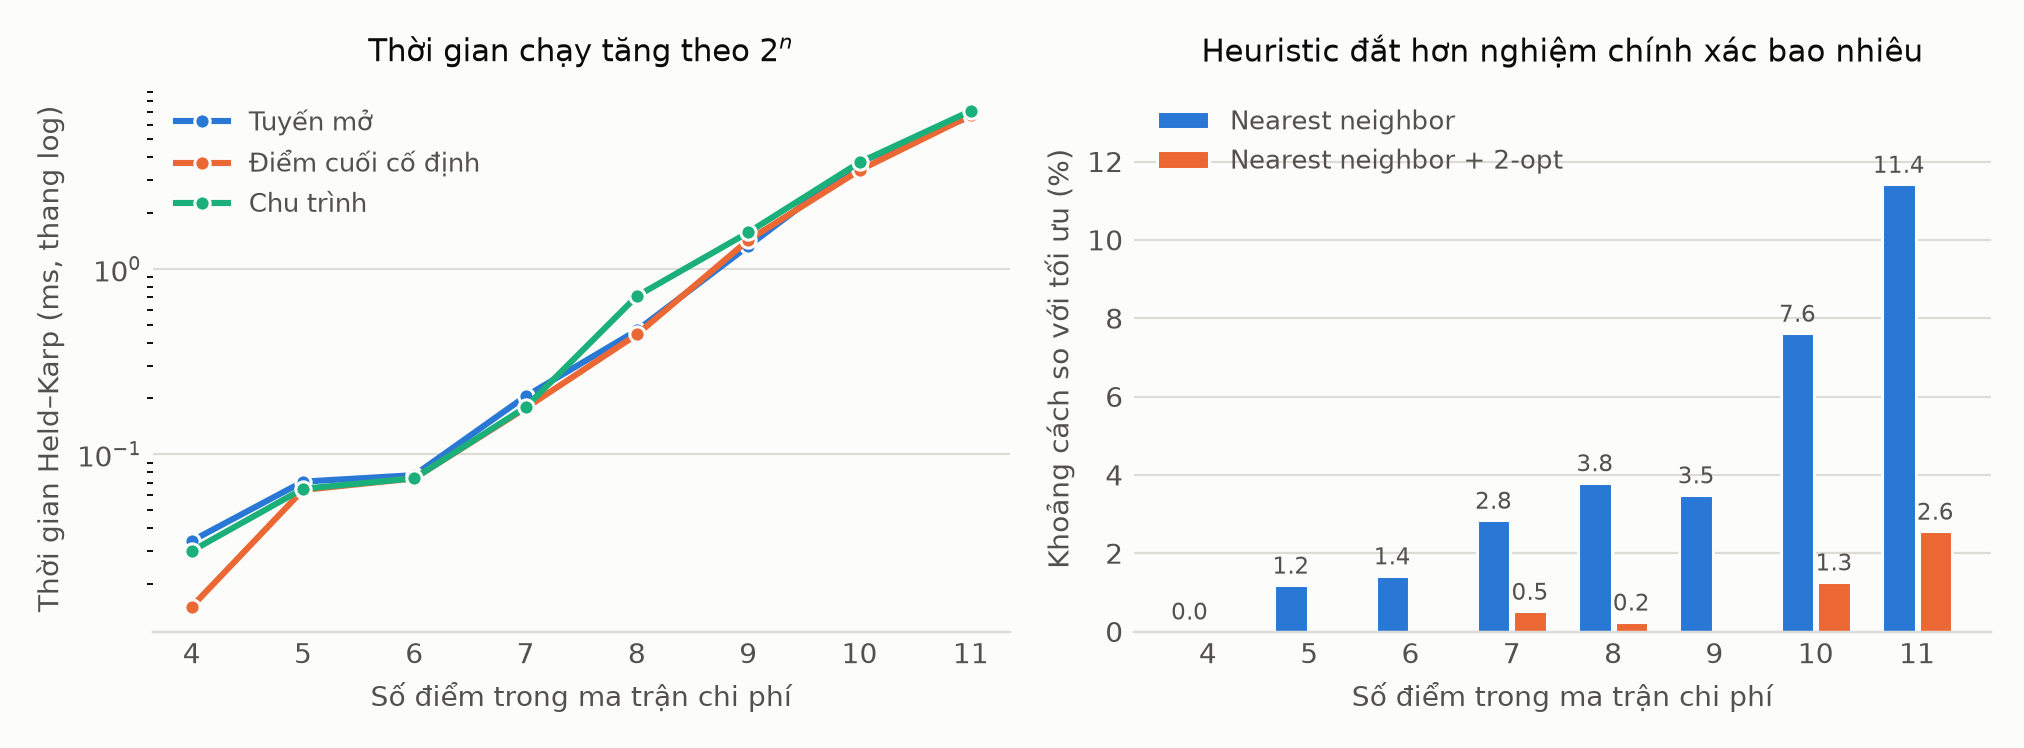
\includegraphics[width=\linewidth]{tsp-scaling.png}
\caption[Thời gian Held--Karp và khoảng cách chất lượng của heuristic]
{Trái: thời gian Held--Karp theo số điểm trên thang log, ba kiểu kết thúc.
Phải: khoảng cách trung bình so với nghiệm tối ưu của hai heuristic}
\label{fig:tsp-scaling}
\end{figure}

\begin{table}[H]
\centering
\small
\caption{Thời gian trung bình của ba thuật toán theo số điểm (kiểu chu trình)}
\label{tab:tsp-runtime}
\begin{tabular}{r r r r r r}
\toprule
\textbf{Điểm} & \textbf{Số trạng thái DP} & \textbf{Held--Karp} &
\textbf{NN} & \textbf{NN + 2-opt} & \textbf{Tỉ lệ tăng} \\
 & $(n-1)2^{\,n-1}$ & (ms) & (ms) & (ms) & Held--Karp \\
\midrule
4 & 24 & 0,030 & 0,008 & 0,019 & -- \\
5 & 64 & 0,065 & 0,009 & 0,039 & 2,17 \\
6 & 160 & 0,074 & 0,005 & 0,029 & 1,14 \\
7 & 384 & 0,179 & 0,007 & 0,041 & 2,42 \\
8 & 896 & 0,712 & 0,012 & 0,075 & 3,98 \\
9 & 2048 & 1,569 & 0,012 & 0,080 & 2,20 \\
10 & 4608 & 3,748 & 0,011 & 0,093 & 2,39 \\
11 & 10240 & 7,113 & 0,013 & 0,115 & 1,90 \\
\bottomrule
\end{tabular}
\end{table}

Cột cuối là tỉ số thời gian giữa hai kích thước liên tiếp. Trung bình nhân của các
tỉ số từ 7 đến 11 điểm là khoảng 2,4 lần cho mỗi điểm thêm vào, nằm quanh mức mà
công thức $O(n^2 2^n)$ dự đoán ở dải này. Hai giá trị nhỏ ở $n=5$ và $n=6$ là
nhiễu đo: ở mức vài chục micro giây, chi phí khởi tạo và dao động bộ đệm lấn át
phần tính toán, nên không nên đọc tỉ lệ tăng tại các kích thước nhỏ nhất.

Điều quan trọng về mặt kỹ thuật là mức tuyệt đối. Ở giới hạn thiết kế 10 điểm cần
ghé (11 điểm trong ma trận), Held--Karp vẫn chỉ tốn khoảng 7 ms, nhỏ hơn hai bậc
độ lớn so với bước lập ma trận chi phí. Nói cách khác, trong phạm vi mà giao diện
cho phép, tầng tổ hợp \textbf{không} phải nút cổ chai; chi phí thực tế nằm ở
Dijkstra trên graph lớn.

\begin{table}[H]
\centering
\caption{Thời gian lập ma trận chi phí bằng Dijkstra theo số điểm}
\label{tab:dijkstra-scaling}
\begin{tabular}{r r r}
\toprule
\textbf{Điểm} & \textbf{Số lần chạy Dijkstra} & \textbf{Thời gian (giây)} \\
\midrule
4 & 4 & 0,484 \\
5 & 5 & 0,806 \\
6 & 6 & 1,462 \\
7 & 7 & 1,618 \\
8 & 8 & 1,649 \\
9 & 9 & 1,860 \\
10 & 10 & 1,995 \\
11 & 11 & 2,218 \\
\bottomrule
\end{tabular}
\end{table}

Thời gian Dijkstra tăng gần tuyến tính theo số điểm chứ không theo giai thừa, vì
mỗi điểm chỉ thêm một lần chạy nguồn đơn nhiều đích. Tỉ lệ giữa hai tầng tại 11
điểm là khoảng $2{,}218$ giây so với $7{,}1$ ms, tức tầng đồ thị chiếm hơn 99,6\%
tổng thời gian tối ưu. Đây là lý do kiến trúc tách hai tầng và cache graph trong
phiên: muốn giảm thời gian chờ thì phải nhắm vào Dijkstra và việc nạp graph, không
phải vào Held--Karp.

\subsection{Diễn giải và giới hạn của phép đo}

Benchmark này cho phép kết luận ba điều trong phạm vi dữ liệu đã dùng: Held--Karp
khả thi về thời gian ở toàn bộ dải được hỗ trợ; nearest-neighbor có thể lệch hai
chữ số phần trăm khi tuyến bị ràng buộc điểm cuối; và 2-opt là một cải thiện rẻ
nhưng không phải một lời bảo đảm.

Giới hạn cần nói rõ: phép đo chỉ dùng một tập 11 địa điểm tại Hà Nội và các tập
con lồng nhau của nó, nên không phải một mẫu ngẫu nhiên của mọi cấu hình điểm. Với
tập điểm cụm chặt hoặc phân bố hình sao, thứ hạng heuristic có thể khác. Thời gian
đo trên một máy phát triển với Python 3.11 và không loại bỏ ảnh hưởng của tải hệ
thống; vì vậy tỉ lệ giữa các tầng đáng tin hơn giá trị tuyệt đối. Cuối cùng, phép
đo tách ma trận chi phí ra khỏi tầng tổ hợp một cách có chủ ý, nên các con số ở
Bảng~\ref{tab:tsp-runtime} không cộng lại thành thời gian người dùng cảm nhận;
Bảng~\ref{tab:dijkstra-scaling} mới là phần chiếm đa số thời gian đó.

\section{Thiết kế benchmark trò chơi}

Mỗi sân dùng 20 seed, ba bot người trốn và ba chiến thuật máy, tạo
$20\times3\times3=180$ ván/sân và 360 ván tổng cộng. Bộ luật cố định:
$b_r=b_h=160$ m, tiết lộ mỗi ba lượt, tối đa 18 lượt. Ba bot người trốn là:
\begin{itemize}
  \item \texttt{random}: chọn ngẫu nhiên trong các nút khả đạt;
  \item \texttt{nearest\_exit}: ưu tiên tiến về lối thoát gần nhất;
  \item \texttt{evasive}: ưu tiên tránh đội máy trong khi vẫn tìm lối thoát.
\end{itemize}

Bot và vị trí khởi đầu đều cố định theo seed. Vì không có người chơi thật, phép
đo chỉ đánh giá tương tác với ba hành vi lập trình sẵn. Không chiến thuật nào
trong hai phía được chứng minh tối ưu.

\section{Kết quả trên sân lưới mô phỏng}

\begin{table}[H]
\centering
\small
\caption{Benchmark sân lưới 81 nút; mỗi dòng gồm 20 ván}
\begin{tabular}{llrrrrrr}
\toprule
\textbf{Bot trốn} & \textbf{Máy} & \textbf{Thoát} & \textbf{Bắt} & \textbf{Hết lượt} &
\textbf{Lượt TB} & \textbf{ms/bước TB} & \textbf{ms max} \\
\midrule
Ngẫu nhiên & Dấu vết & 3 & 16 & 1 & 6,15 & 0,724 & 3,470 \\
Ngẫu nhiên & Tìm kiếm & 2 & 18 & 0 & 4,45 & 0,882 & 3,523 \\
Ngẫu nhiên & Phối hợp & 1 & 19 & 0 & 4,80 & 3,973 & 14,897 \\
Gần lối thoát & Dấu vết & 18 & 2 & 0 & 3,15 & 0,628 & 2,806 \\
Gần lối thoát & Tìm kiếm & 19 & 1 & 0 & 3,20 & 0,870 & 2,828 \\
Gần lối thoát & Phối hợp & 13 & 7 & 0 & 3,20 & 2,972 & 10,620 \\
Né tránh & Dấu vết & 19 & 1 & 0 & 3,90 & 0,589 & 3,147 \\
Né tránh & Tìm kiếm & 20 & 0 & 0 & 3,70 & 1,119 & 3,345 \\
Né tránh & Phối hợp & 19 & 1 & 0 & 4,50 & 3,304 & 11,581 \\
\bottomrule
\end{tabular}
\end{table}

Trên bot ngẫu nhiên, phối hợp bắt 19/20 ván, cao hơn dấu vết 16/20. Trên bot đi
thẳng tới lối thoát, phối hợp bắt 7/20, trong khi hai chiến thuật còn lại chỉ bắt
2/20 và 1/20. Đây là bằng chứng cấu hình cụ thể cho lợi ích của thành phần chặn
lối thoát. Tuy nhiên bot né tránh vẫn thoát 19/20 trước phối hợp. Tổng trên 60
ván/chiến thuật, phối hợp bắt 27 ván, còn dấu vết và tìm kiếm cùng bắt 19 ván.

Đổi lại, phối hợp tốn 2,972--3,973 ms/bước trung bình, cao hơn các chính sách đơn
dưới 1,2 ms ở phần lớn cấu hình. Mức này vẫn phù hợp tương tác, nhưng phản ánh chi
phí xét tổ hợp ứng viên giữa hai đội.

\section{Kết quả trên sân OSM cục bộ}

\begin{table}[H]
\centering
\small
\caption{Benchmark sân OSM 358 nút; mỗi dòng gồm 20 ván}
\begin{tabular}{llrrrrrr}
\toprule
\textbf{Bot trốn} & \textbf{Máy} & \textbf{Thoát} & \textbf{Bắt} & \textbf{Hết lượt} &
\textbf{Lượt TB} & \textbf{ms/bước TB} & \textbf{ms max} \\
\midrule
Ngẫu nhiên & Dấu vết & 0 & 20 & 0 & 8,25 & 2,026 & 11,804 \\
Ngẫu nhiên & Tìm kiếm & 0 & 20 & 0 & 7,95 & 2,580 & 10,702 \\
Ngẫu nhiên & Phối hợp & 0 & 19 & 1 & 9,30 & 5,241 & 18,427 \\
Gần lối thoát & Dấu vết & 16 & 4 & 0 & 6,30 & 2,137 & 11,864 \\
Gần lối thoát & Tìm kiếm & 15 & 5 & 0 & 5,95 & 2,297 & 8,666 \\
Gần lối thoát & Phối hợp & 16 & 4 & 0 & 6,15 & 4,255 & 12,369 \\
Né tránh & Dấu vết & 15 & 1 & 4 & 9,65 & 1,816 & 8,055 \\
Né tránh & Tìm kiếm & 15 & 1 & 4 & 9,90 & 2,273 & 8,620 \\
Né tránh & Phối hợp & 13 & 2 & 5 & 9,85 & 3,716 & 11,151 \\
\bottomrule
\end{tabular}
\end{table}

Trên sân OSM, cả ba chiến thuật bắt toàn bộ hoặc gần toàn bộ bot ngẫu nhiên.
Với bot gần lối thoát, số ván bắt chỉ từ 4 đến 5; với bot né tránh, chỉ từ 1 đến
2, còn 4--5 ván kết thúc do hết lượt. Tổng số bắt trên 60 ván lần lượt là 25,
26 và 25 cho dấu vết, tìm kiếm và phối hợp. Vì vậy benchmark này bác bỏ cách diễn
giải đơn giản rằng phối hợp luôn mạnh nhất.

Sự khác biệt giữa sân lưới và OSM có thể do topology, vị trí lối thoát, đường cụt
và shortlist ứng viên, nhưng benchmark hiện tại chưa cô lập nguyên nhân. Đây là
giả thuyết cần thí nghiệm ablation, không phải kết luận đã kiểm chứng.

\begin{figure}[H]
\centering
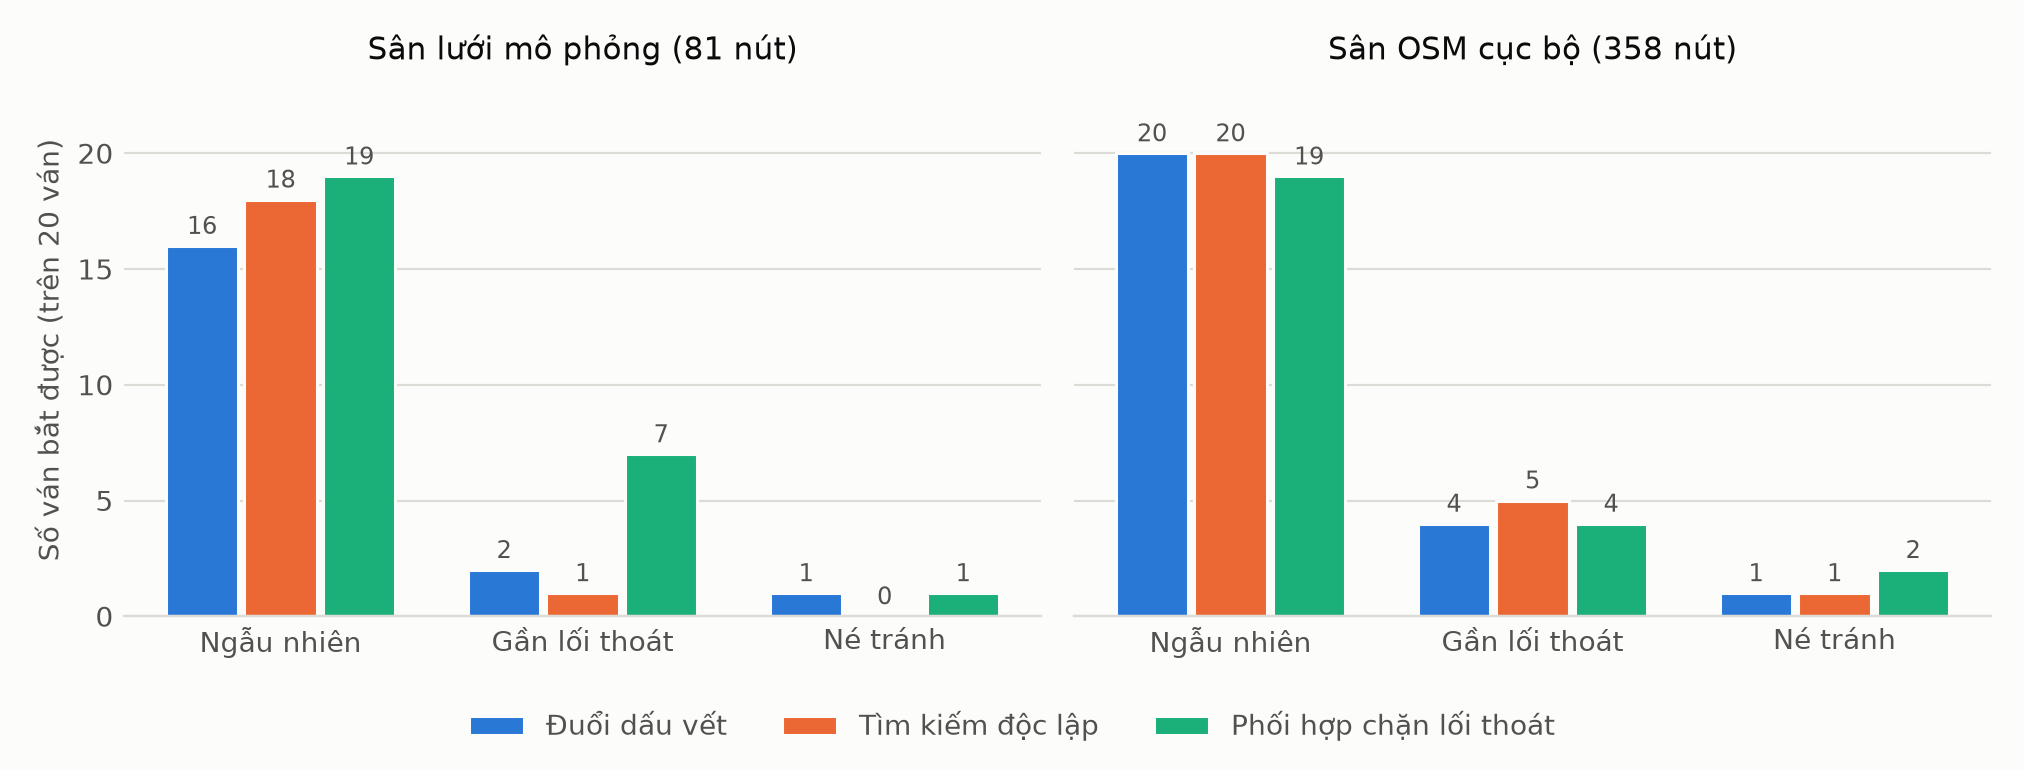
\includegraphics[width=\linewidth]{benchmark-capture.png}
\caption[Số ván bắt được theo chiến thuật máy và bot người trốn]
{Số ván bắt được trên mỗi cấu hình 20 ván, đối chiếu hai sân. Thứ hạng ba chiến
thuật đảo khi đổi sân và đổi bot người trốn}
\label{fig:benchmark-capture}
\end{figure}

Hình~\ref{fig:benchmark-capture} đặt hai sân cạnh nhau để thấy rõ điều mà hai bảng
số rời rạc dễ che: lợi thế của chiến thuật phối hợp chỉ xuất hiện ở sân lưới và
chỉ với hai trong ba bot, còn trên sân OSM ba cột gần như bằng nhau ở mọi nhóm.
Nếu một chiến thuật thực sự trội, các cột xanh lục phải cao hơn ở cả sáu nhóm;
dữ liệu không cho thấy điều đó.

\section{Đánh giá giao diện và tích hợp}

AppTest kiểm tra mở mặc định ở Lộ trình, deep link tới Trốn tìm, chuyển qua lại
và giữ tiêu chí/kiểu điểm cuối/click bản đồ. Các kịch bản game đi đến ba kết cục
\texttt{escaped}, \texttt{caught}, \texttt{timeout}. Playwright được dùng để
kiểm tra trình duyệt thật: chọn Hồ Hoàn Kiếm tới Nhà hát Lớn, tối ưu được tuyến
1,36 km với thời gian hiển thị 1,4 phút; chuyển sang trò chơi rồi quay lại vẫn
giữ nguyên kết quả.

\begin{figure}[H]
\centering
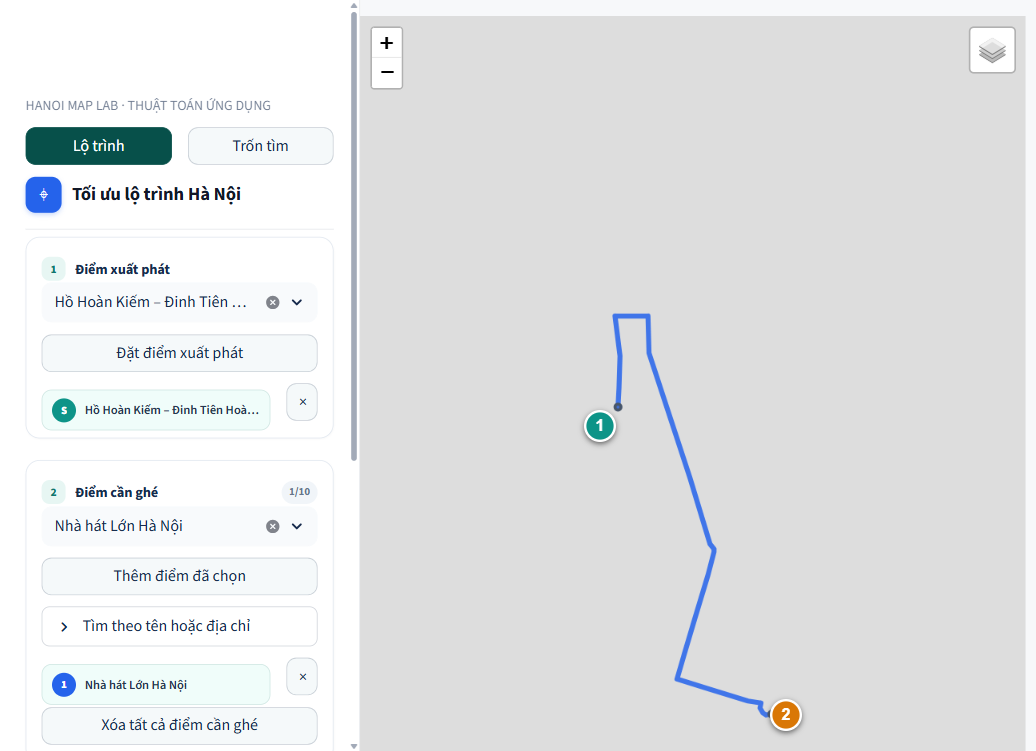
\includegraphics[width=0.92\linewidth]{route-result.png}
\caption{Tuyến thực được vẽ sau khi tối ưu trong giao diện tích hợp}
\label{fig:route-result}
\end{figure}

Trong ảnh kiểm tra, tile nền màu xám do sự cố phân giải/chính sách mạng của máy
thử nghiệm, nhưng polyline và chỉ số thuật toán vẫn hiển thị. Điều này minh họa
việc tile nền và graph định tuyến là hai thành phần độc lập.

\section{Các mối đe dọa tới tính hợp lệ}

\textbf{Tính hợp lệ nội tại:} benchmark dùng cùng seed giữa các chiến thuật, nhưng
không thực hiện kiểm định thống kê hoặc hoán đổi ngẫu nhiên thứ tự chạy. Thời gian
có thể bị ảnh hưởng bởi warm cache và tải hệ thống.

\textbf{Tính hợp lệ cấu trúc:} tỉ lệ bắt/thoát đo hiệu quả trong luật trò chơi đã
định nghĩa, không đo chất lượng chiến thuật trong pursuit--evasion liên tục. Hàm
coverage là proxy khoảng cách, không phải xác suất bắt.

\textbf{Tính hợp lệ ngoại suy:} chỉ có hai sân, ba bot và 20 seed. Sân OSM là
phần graph cục bộ đã điều chỉnh hai chiều. Không thể suy ra hiệu quả trên toàn Hà
Nội, người chơi thật hoặc điều kiện giao thông thực tế.

\textbf{Tính đúng dữ liệu:} trọng số thời gian là ước tính tĩnh. Kết quả 29,93
phút không phải dự báo thời gian thực và không nên dùng như chỉ dẫn giao thông.
